\documentclass[conference]{IEEEtran}
\IEEEoverridecommandlockouts
% The preceding line is only needed to identify funding in the first footnote. If that is unneeded, please comment it out.
%Template version as of 6/27/2024

\usepackage[T1]{fontenc}
\usepackage[utf8]{inputenc}
\usepackage[croatian]{babel}
\usepackage{cite}
\usepackage{amsmath,amssymb,amsfonts}
\usepackage{algorithmic}
\usepackage{graphicx}
\usepackage{textcomp}
\usepackage{xcolor}
\usepackage{tikz}
\usepackage{relsize}
\usepackage{calc}
\usepackage{paralist}
\usepackage{import}
\usepackage{float}
\usepackage{multirow}

\usetikzlibrary{shapes.multipart, calc}

\def\BibTeX{{\rm B\kern-.05em{\sc i\kern-.025em b}\kern-.08em
    T\kern-.1667em\lower.7ex\hbox{E}\kern-.125emX}}
    
\tikzset{fontscale/.style = {font=\relsize{#1}}
    }

\subimport{../layers/}{init}
\usetikzlibrary{positioning}
\usetikzlibrary{3d} %for including external image 


\def\ConvColor{rgb:yellow,5;red,2.5;white,5}
\def\ConvReluColor{rgb:yellow,5;red,5;white,5}
\def\PoolColor{rgb:red,1;black,0.3}
\def\UnpoolColor{rgb:blue,2;green,1;black,0.3}
\def\FcColor{rgb:blue,5;red,2.5;white,5}
\def\FcReluColor{rgb:blue,5;red,5;white,4}
\def\SoftmaxColor{rgb:magenta,5;black,7}   
\def\SumColor{rgb:blue,5;green,15}


\newcommand{\copymidarrow}{\tikz \draw[-Stealth,line width=0.8mm,draw={rgb:blue,4;red,1;green,1;black,3}] (-0.3,0) -- ++(0.3,0);}
 
    
\begin{document}

\title{Prepoznavanje umjetno (AI) generiranih slika\\}

\author{
\IEEEauthorblockN{Paula Močinić}
\IEEEauthorblockA{\textit{Računarska znanost} \\
\textit{FER}\\
paula.mocinic@fer.hr}
\and
\IEEEauthorblockN{Mihael Pristav}
\IEEEauthorblockA{\textit{Računarska znanost} \\
\textit{FER}\\
mihael.pristav@fer.hr}
\and
\IEEEauthorblockN{Fran Lubina}
\IEEEauthorblockA{\textit{Računarska znanost} \\
\textit{FER}\\
fran.lubina@fer.hr}
\and
\IEEEauthorblockN{Ante Čavar}
\IEEEauthorblockA{\textit{Računarska znanost} \\
\textit{FER}\\
ante.cavar@fer.hr}
}

\maketitle

\begin{abstract}
Ovaj dokument prikazuje naš proces i istraživanje kroz koje objašnjavamo na koji način
smo razvili model koji prepoznaje AI generirane slike.
\end{abstract}

\begin{IEEEkeywords}
AI, deep-fake, perceptron
\end{IEEEkeywords}

\section{Uvod}Zadnjih par godina svjedočimo nevjerojatnom napretku generativnih modela poput GAN-ova i difuzijskih modela (npr. Stable Diffusion i Midjourney), koji su podigli kvalitetu umjetno generiranih slika na razinu koju je ljudskom oku gotovo nemoguće razlikovati od stvarnosti. Iako ova tehnologija nudi goleme kreativne mogućnosti, ona donosi i ozbiljne izazove u području digitalne forenzike i provjere informacija, jer se lažni vizualni sadržaji mogu lako koristiti za manipulaciju javnim mnijenjem ili krađu identiteta. U ovom projektu fokusirali smo se na razvoj sustava za automatsko prepoznavanje AI generiranih slika koristeći duboko učenje. Naš cilj je istražiti možemo li pomoću specifičnih arhitektura neuronskih mreža pouzdano "uhvatiti" suptilne tragove koje generativni procesi ostavljaju u pikselima.

\subsection{Opis problema}Glavni zadatak koji rješavamo je binarna klasifikacija: moramo odrediti pripada li ulazna slika klasi "stvarnih" ili "AI generiranih" slika. Iako to na papiru zvuči jednostavno, u praksi je vrlo izazovno jer moderni generatori više ne ostavljaju očite pogreške u teksturama ili frekvencijskom spektru, što je ranije bio glavni način detekcije. Također, modeli moraju biti sposobni prepoznati slike iz različitih izvora, a ne samo iz onih na kojima su trenirani.

\subsection{Motivacija}Glavni pokretač za ovaj rad je činjenica da povjerenje u digitalne medije rapidno opada. Željeli smo stvoriti alat koji bi mogao služiti kao pomoć pri moderiranju sadržaja na online platformama.

\section{Pregled literature}
\label{sect:litrev}
Pregledom dosadašnjih radova vidjeli smo da su konvolucijske neuronske mreže (CNN) i dalje "zlatni standard" za ovaj problem zbog svoje sposobnosti da izvuku lokalne značajke i teksturalne anomalije. Modeli poput ResNet-50 i EfficientNet-a često postižu točnost veću od 90\% na standardnim skupovima podataka kao što je CIFAKE. Međutim, literatura također naglašava jedan veliki problem: generalizaciju. Modeli koji savršeno rade na slikama iz jednog generatora često potpuno zakazuju kada im se podmetne slika iz novijeg ili drugačijeg modela. Novija istraživanja sugeriraju da bi rješenje moglo biti u promjeni klasifikacijske glave – na primjer, zamjenom standardnog Softmax sloja s SVM (Support Vector Machine) klasifikatorom, što u nekim slučajevima daje robusnije rezultate na rubnim primjerima.

\section{Rješenje}

\subsection{Opis i metodologija rada}
\label{sect:metoda}
Naše rješenje temelji se na usporedbi dvije varijante CNN modela. Oba modela koriste sličnu "okosnicu" za ekstrakciju značajki, ali se razlikuju u načinu donošenja konačne odluke:
CNN s Softmax slojem: Klasičan pristup koji koristi kros-entropijsku funkciju gubitka i daje nam vjerojatnost pripadnosti klasi.
Hibridni CNN-SVM model: Ovdje smo zadnji sloj mreže zamijenili SVM-om s linearnim kernelom. SVM pokušava maksimizirati marginu između stvarnih i lažnih slika u prostoru značajki koji je mreža naučila, što bi trebalo donijeti bolju separaciju klasa.

\subsection{Opis rješenja}
CNN koji smo koristili ima arhitekturu, odnosno slojeve kao na slici \ref{pic:CNN_layers}.


Kao što je već ranije spomenuto (cjelina \ref{sect:metoda}) "okosnica", odnosno svi slojevi prije sloja za vektorizaciju je zajednički za sve modele. Kod CNN-SVM hibridne inačice se svi slojevi nakon toga jednostavno zamijene SVM-om. To je pak prikazano na slici \ref{pic:CNN_SVM_layers}

\subsection{Optimizacija i treniranje}Da bismo izvukli maksimum iz oba modela, nismo nasumično birali parametre, već smo proveli Grid Search optimizaciju. Kod SVM-a smo sustavno varirali parametar regularizacije $C$ i parametar $\gamma$ (gamma) kako bismo pronašli idealan kompromis između točnosti na trening setu i sposobnosti generalizacije na novim podacima.Modeli su trenirani na CIFAKE datasetu koji sadrži 120,000 slika, što nam je osiguralo dovoljno veliku i balansiranu bazu za učenje. 

Pri razvoju smo koristili:
\begin{enumerate}
\item Podjelu 8:72:20 za CNN inačicu
\item Podjelu 80:20 za SVM dio CNN-SVM Inačice.
\end{enumerate}
Za obje inačice prvotni ispitni skup dijelimo na skup za skup za učenje i skup za testiranje u omjeru 80:20, za učenje CNN (što uključuje i "okosnicu" iz cjeline \ref{sect:metoda}) se daj skup dodatno dijeli u omjeru 90:10 na skup za učenje i skup za validaciju.


Slike su prije ulaza u mrežu normalizirane i skalirane na fiksnu rezoluciju (npr. $224 \times 224$ piksela) kako bi proces učenja bio stabilniji i brži. Uspjeh mjerimo kroz točnost (accuracy), ali i kroz konfuzijsku matricu kako bismo točno vidjeli koji tip slika model najčešće griješi.


\subsection{Opis eksperimentalnih rezultata}
Rezultati su dobiveni na podskupu CIFAKE skupa za testiranje (20k slika, 10k po kategoriji).

\begin{tabular}{|p{50pt}|p{30pt}|p{30pt}|p{30pt}|p{30pt}|}
	\hline
	\textbf{model} & \textbf{acc.} & \textbf{prec.} & \textbf{recall} & \textbf{f1-score}\\
	\hline
	CNN & 93.25\% & 0.90 & 0.97 & 0.94\\ \hline
	CNN + SVM(linear) & 94.31\% & 0.94 & 0.95 & 0.94\\ \hline
	CNN + SVM(RBF) & 94.59\% & 0.95 & 0.95 & 0.95\\ \hline
\end{tabular}
\ \\
Odnosno, kada bi grafički prikazali točnost za sva tri modela:

\begin{figure}[H]
\centering
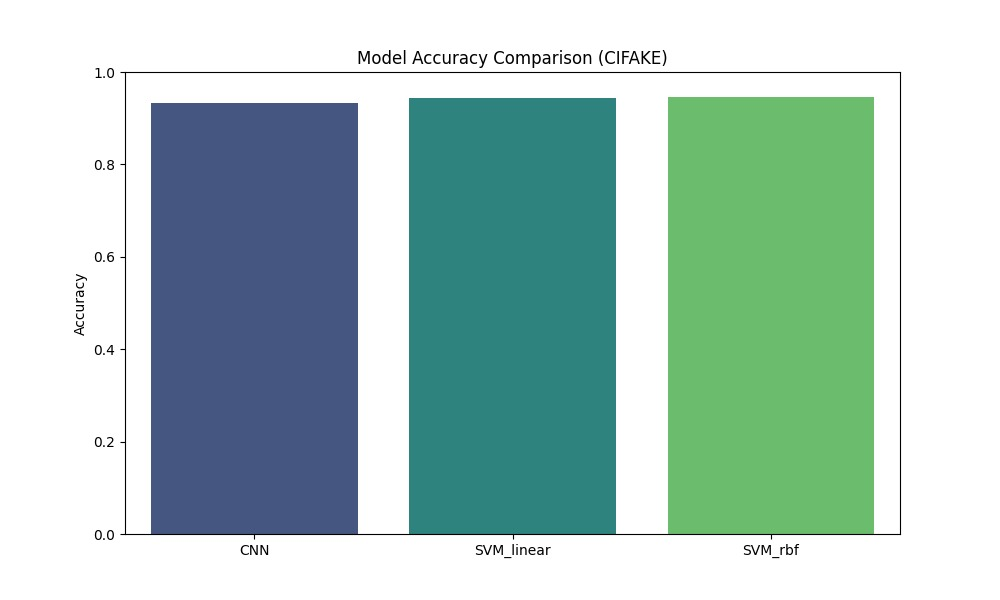
\includegraphics[scale=0.28]{../pics/acc_chart.jpg}\\

\end{figure}
\ \\
\begin{figure}[H]
\centering
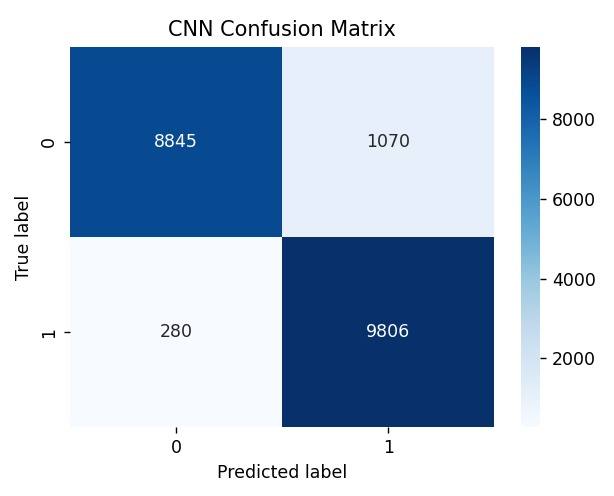
\includegraphics[scale=0.28]{../pics/cnn_conf.png}\\

\end{figure}
\ \\
\begin{figure}[H]
\centering
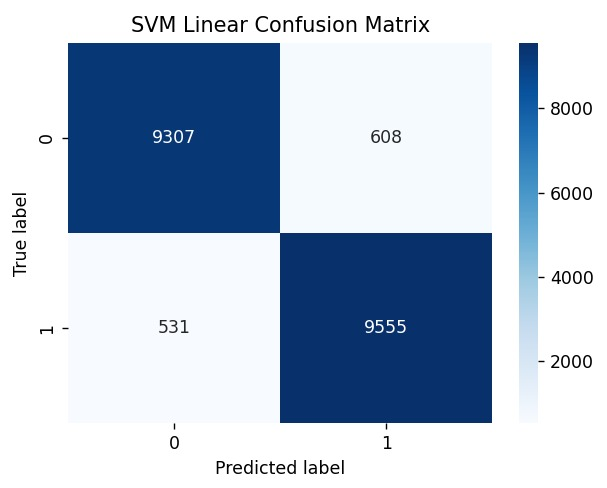
\includegraphics[scale=0.28]{../pics/linear_conf.png}\\

\end{figure}
\ \\
\begin{figure}[H]
\centering
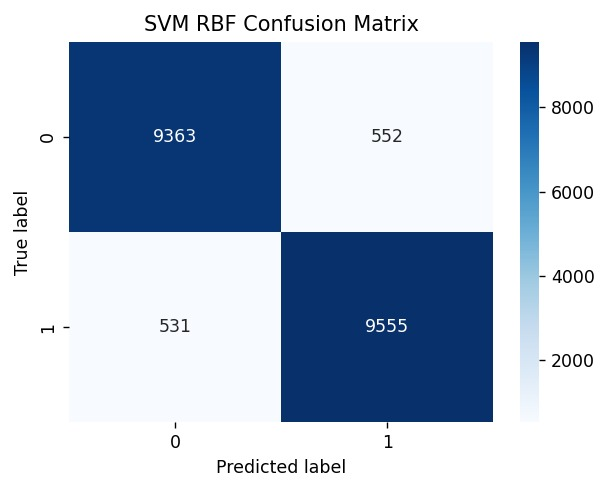
\includegraphics[scale=0.28]{../pics/rbf_conf.png}\\

\end{figure}

\section{Diskusija}

\subsection{O našim rezultatima}
\label{sect:ourres}
Na grafu točnosti vidimo da modeli svi imaju vrlo sličnu točnost. Što je i za očekivati obzirom da dijele većinu arhitekture. Samo je način donošenja odluke drugačiji nakon što su slike već vektorizirane. Također vidimo da CNN-SVM sa RBF kernelom ima najveću točnost. Autori misle da je razlogu tomu: 
\begin{inparaenum}\item Krutost linearnog kernela \item dodatni hiperparametar kod RBF kernela (preciznost) \end{inparaenum}.
No detaljnija analiza nadilazi opseg i ciljeve ovog izvještaja.\\
U cjelini \ref{sect:litrev} je rečeno da je CNN "zlatni standard" za ovakve probleme. No vidimo da je moguće dobiti i bolje rezultate ako se izgradi mreža koja zadržava svu moć vektorizacije slike koju nude ulazni slojevi CNN mreža te se još k tome doda model strojnog učenja koji bolje klasificira primjere neko gusti slojevi.


\subsection{Usporedba sa literaturom}
Rezultati su vrlo slični, barem sa usporedivim arhitekturama, što je i za očekivati obzirom da je arhitektura mreže gotovo identična te da su skupovi podataka
slične veličine. Naša mreža, napose SVM sa RBF kernelom ima nešto bolji rezultat. To je vjerojatno zbog poboljšane mogućnosti klasifikacije
koju nudi kernel-SVM u odnosu na guste slojeve te zbog razloga navedenih u cjelini \ref{sect:ourres}.

\begin{tabular}{|p{50pt}|p{50pt}|p{30pt}|p{25pt}|p{25pt}|p{25pt}|}
	\hline
	\textbf{model} & \textbf{dataset} & \textbf{acc.} & \textbf{prec} & \textbf{recall} & \textbf{f1-score}\\
	\hline
	CvT [1] & ArtiFact & 98.54\% & 0.99 & 0.98 & 0.98\\ \hline
	CNN [2] & Kaggle ai-get-img, CIFAKE, pygoogle & 93.9\% & 0.97 & 0.91 & 0.94\\ \hline
	ViT [3] & CIFAKE & 98.25\% & 0.99 & 0.98 & 0.98\\ \hline
\end{tabular}
\ \\
Međutim naši rezultati su znatno lošiji od novijih modela kao što su ViT transformatori ili modeli bazirani na njima (CvT). Transformatori bolje zadržavaju podatke nakon dugih sekvenci, odnosno između udaljenih piksela na istoj slici. Globalni uzorci se bolje raspoznavaju nego kod konvolucijskih mreža, bez gubitka kvalitete prepoznavanja lokalnih uzoraka.


\section{arhitektura CNN}
\label{pic:CNN_layers}
\ \\
\\
\\
\begin{tikzpicture}[scale=0.5,rotate=90,transform shape]s
\tikzstyle{connection}=[ultra thick,every node/.style={sloped,allow upside down},draw=\edgecolor,opacity=0.7]
\tikzstyle{copyconnection}=[ultra thick,every node/.style={sloped,allow upside down},draw={rgb:blue,4;red,1;green,1;black,3},opacity=0.7]

\node[canvas is zy plane at x=0] (temp) at (-1,0,0) {
\includegraphics[width=13cm,height=13cm]{../pics/fer_logo.jpg}};

\pic[shift={(0,0,0)}] at (0,0,0) 
    {Box={
        name=conv1,
        caption=Conv2D 32,
        xlabel={{32, }},
        zlabel=128,
        fill=\ConvColor,
        height=64,
        width=2,
        depth=64
        }
    };


\pic[shift={ (0,0,0) }] at (conv1-east) 
    {Box={
        name=pool1,
        caption=MaxPool,
        fill=\PoolColor,
        opacity=0.5,
        height=32,
        width=1,
        depth=32
        }
    };


\pic[shift={(1.5,0,0)}] at (pool1-east) 
    {Box={
        name=conv2,
        caption=Conv2D 64,
        xlabel={{64, }},
        zlabel=64,
        fill=\ConvColor,
        height=32,
        width=4,
        depth=32
        }
    };


\draw [connection]  (pool1-east)    -- node {\midarrow} (conv2-west);


\pic[shift={ (0,0,0) }] at (conv2-east) 
    {Box={
        name=pool2,
        caption=MaxPool,
        fill=\PoolColor,
        opacity=0.5,
        height=16,
        width=1,
        depth=16
        }
    };


\pic[shift={(1.5,0,0)}] at (pool2-east) 
    {Box={
        name=conv3,
        caption=Conv2D 128,
        xlabel={{128, }},
        zlabel=32,
        fill=\ConvColor,
        height=16,
        width=6,
        depth=16
        }
    };


\draw [connection]  (pool2-east)    -- node {\midarrow} (conv3-west);


\pic[shift={ (0,0,0) }] at (conv3-east) 
    {Box={
        name=pool3,
        caption=MaxPool,
        fill=\PoolColor,
        opacity=0.5,
        height=8,
        width=1,
        depth=8
        }
    };


\pic[shift={(1.5,0,0)}] at (pool3-east) 
    {Box={
        name=conv4,
        caption=Conv2D 256,
        xlabel={{256, }},
        zlabel=16,
        fill=\ConvColor,
        height=8,
        width=8,
        depth=8
        }
    };


\draw [connection]  (pool3-east)    -- node {\midarrow} (conv4-west);


\pic[shift={ (0,0,0) }] at (conv4-east) 
    {Box={
        name=pool4,
        caption=MaxPool,
        fill=\PoolColor,
        opacity=0.5,
        height=4,
        width=1,
        depth=4
        }
    };


\pic[shift={(1.5,0,0)}] at (pool4-east) 
    {Box={
        name=flat,
        caption=Vektorizacija,
        xlabel={{1, }},
        zlabel=1,
        fill=\ConvColor,
        height=32,
        width=1,
        depth=1
        }
    };


\draw [connection]  (pool4-east)    -- node {\midarrow} (flat-west);


\pic[shift={(2,0,0)}] at (flat-east) 
    {Box={
        name=dense1,
        caption=Gusti 64,
        xlabel={{64, }},
        zlabel=1,
        fill=\ConvColor,
        height=24,
        width=1.5,
        depth=1
        }
    };


\draw [connection]  (flat-east)    -- node {\midarrow} (dense1-west);


\pic[shift={(2,0,0)}] at (dense1-east) 
    {Box={
        name=dense2,
        caption=Gusti 64,
        xlabel={{64, }},
        zlabel=1,
        fill=\ConvColor,
        height=24,
        width=1.5,
        depth=1
        }
    };


\draw [connection]  (dense1-east)    -- node {\midarrow} (dense2-west);


\pic[shift={(1,0,0)}] at (dense2-east) 
    {Box={
        name=output,
        caption=Sigmoid (Izlaz),
        xlabel={{" ","dummy"}},
        zlabel=1,
        fill=\SoftmaxColor,
        opacity=0.8,
        height=10,
        width=1,
        depth=1
        }
    };


\draw [connection]  (dense2-east)    -- node {\midarrow} (output-west);


\end{tikzpicture} 



\section{arhitektura CNN-SVM}
\label{pic:CNN_SVM_layers}
\ \\
\\
\\
\begin{tikzpicture}[scale=0.5,rotate=90,transform shape]
\tikzstyle{connection}=[ultra thick,every node/.style={sloped,allow upside down},draw=\edgecolor,opacity=0.7]
\tikzstyle{copyconnection}=[ultra thick,every node/.style={sloped,allow upside down},draw={rgb:blue,4;red,1;green,1;black,3},opacity=0.7]

\node[canvas is zy plane at x=0] (temp) at (-1,0,0) {
\includegraphics[width=13cm,height=13cm]{../pics/fer_logo.jpg}};

\pic[shift={(0,0,0)}] at (0,0,0) 
    {Box={
        name=conv1,
        caption=Conv2D 32,
        xlabel={{32, }},
        zlabel=128,
        fill=\ConvColor,
        height=64,
        width=2,
        depth=64
        }
    };


\pic[shift={ (0,0,0) }] at (conv1-east) 
    {Box={
        name=pool1,
        caption=MaxPool,
        fill=\PoolColor,
        opacity=0.5,
        height=32,
        width=1,
        depth=32
        }
    };


\pic[shift={(1.5,0,0)}] at (pool1-east) 
    {Box={
        name=conv2,
        caption=Conv2D 64,
        xlabel={{64, }},
        zlabel=64,
        fill=\ConvColor,
        height=32,
        width=4,
        depth=32
        }
    };


\draw [connection]  (pool1-east)    -- node {\midarrow} (conv2-west);


\pic[shift={ (0,0,0) }] at (conv2-east) 
    {Box={
        name=pool2,
        caption=MaxPool,
        fill=\PoolColor,
        opacity=0.5,
        height=16,
        width=1,
        depth=16
        }
    };


\pic[shift={(1.5,0,0)}] at (pool2-east) 
    {Box={
        name=conv3,
        caption=Conv2D 128,
        xlabel={{128, }},
        zlabel=32,
        fill=\ConvColor,
        height=16,
        width=6,
        depth=16
        }
    };


\draw [connection]  (pool2-east)    -- node {\midarrow} (conv3-west);


\pic[shift={ (0,0,0) }] at (conv3-east) 
    {Box={
        name=pool3,
        caption=MaxPool,
        fill=\PoolColor,
        opacity=0.5,
        height=8,
        width=1,
        depth=8
        }
    };


\pic[shift={(1.5,0,0)}] at (pool3-east) 
    {Box={
        name=conv4,
        caption=Conv2D 256,
        xlabel={{256, }},
        zlabel=16,
        fill=\ConvColor,
        height=8,
        width=8,
        depth=8
        }
    };


\draw [connection]  (pool3-east)    -- node {\midarrow} (conv4-west);


\pic[shift={ (0,0,0) }] at (conv4-east) 
    {Box={
        name=pool4,
        caption=MaxPool,
        fill=\PoolColor,
        opacity=0.5,
        height=4,
        width=1,
        depth=4
        }
    };


\pic[shift={(1.5,0,0)}] at (pool4-east) 
    {Box={
        name=flat,
        caption=Vektorizacija,
        xlabel={{1, }},
        zlabel=1,
        fill=\ConvColor,
        height=32,
        width=1,
        depth=1
        }
    };


\draw [connection]  (pool4-east)    -- node {\midarrow} (flat-west);

\draw [connection]  (flat-west)    -- node {\midarrow} (11.5, 0);

\draw [black, fill=lightgray] ++(11.5,-3) rectangle ++(3.5,6) node[pos=.5, fontscale=3] {SVM};

\end{tikzpicture} 



\section*{Literatura}

[1] Guyfloki (2023). AI Image Detector. GitHub.
https://github.com/guyfloki/ai-image-detector

[2] SanKolisetty (2023). AI Image Classifier. GitHub.
https://github.com/SanKolisetty/AI-Image-Classifier

[3] Dima806 (2024). CiFake: AI-Generated Image Detection with ViT. Kaggle.
https://www.kaggle.com/code/dima806/cifake-ai-generated-image-detection-vit

[4] Yu, Z., Li, X., Zhang, Z., Wang, Y. (2023). On the detection of AI-generated images. arXiv.
https://arxiv.org/abs/2302.11970

[5] GeeksforGeeks (2025). Convolutional Vision Transformer.
https://www.geeksforgeeks.org/computer-vision/convolutional-vision-transformer/

[6] Wikipedia contributors. Vision transformer. Wikipedia.
https://en.wikipedia.org/wiki/Vision\_transformer

[7] Wikipedia contributors. Convolutional neural network. Wikipedia.
https://en.wikipedia.org/wiki/Convolutional\_neural\_network

[8] GeeksforGeeks (2025). Introduction to Convolutional Neural Network.
https://www.geeksforgeeks.org/machine-learning/introduction-convolution-neural-network/

[9] Shervine, S. (2025). CS230: Convolutional Neural Networks Cheatsheet. Stanford University.
https://stanford.edu/~shervine/teaching/cs-230/cheatsheet-convolutional-neural-networks

[10] Dosovitskiy, A., Beyer, L., Kolesnikov, A., Weissenborn, D., Zhai, X., Unterthiner, T., Houlsby, N. (2020).
An image is worth 16x16 words: Transformers for image recognition at scale. arXiv.
https://arxiv.org/abs/2010.11929


% Please number citations consecutively within brackets \cite{b1}. The
% sentence punctuation follows the bracket \cite{b2}. Refer simply to the reference 
% number, as in \cite{b3}---do not use ``Ref. \cite{b3}'' or ``reference \cite{b3}'' except at 
% the beginning of a sentence: ``Reference \cite{b3} was the first $\ldots$''

% Number footnotes separately in superscripts. Place the actual footnote at 
% the bottom of the column in which it was cited. Do not put footnotes in the 
% abstract or reference list. Use letters for table footnotes.

% Unless there are six authors or more give all authors' names; do not use 
% ``et al.''. Papers that have not been published, even if they have been 
% submitted for publication, should be cited as ``unpublished'' \cite{b4}. Papers 
% that have been accepted for publication should be cited as ``in press'' \cite{b5}. 
% Capitalize only the first word in a paper title, except for proper nouns and 
% element symbols.

% For papers published in translation journals, please give the English 
% citation first, followed by the original foreign-language citation \cite{b6}.

% \begin{thebibliography}{00}
% \bibitem{b1} G. Eason, B. Noble, and I. N. Sneddon, ``On certain integrals of Lipschitz-Hankel type involving products of Bessel functions,'' Phil. Trans. Roy. Soc. London, vol. A247, pp. 529--551, April 1955.
% \bibitem{b2} J. Clerk Maxwell, A Treatise on Electricity and Magnetism, 3rd ed., vol. 2. Oxford: Clarendon, 1892, pp.68--73.
% \bibitem{b3} I. S. Jacobs and C. P. Bean, ``Fine particles, thin films and exchange anisotropy,'' in Magnetism, vol. III, G. T. Rado and H. Suhl, Eds. New York: Academic, 1963, pp. 271--350.
% \bibitem{b4} K. Elissa, ``Title of paper if known,'' unpublished.
% \bibitem{b5} R. Nicole, ``Title of paper with only first word capitalized,'' J. Name Stand. Abbrev., in press.
% \bibitem{b6} Y. Yorozu, M. Hirano, K. Oka, and Y. Tagawa, ``Electron spectroscopy studies on magneto-optical media and plastic substrate interface,'' IEEE Transl. J. Magn. Japan, vol. 2, pp. 740--741, August 1987 [Digests 9th Annual Conf. Magnetics Japan, p. 301, 1982].
% \bibitem{b7} M. Young, The Technical Writer's Handbook. Mill Valley, CA: University Science, 1989.
% \bibitem{b8} D. P. Kingma and M. Welling, ``Auto-encoding variational Bayes,'' 2013, arXiv:1312.6114. [Online]. Available: https://arxiv.org/abs/1312.6114
% \bibitem{b9} S. Liu, ``Wi-Fi Energy Detection Testbed (12MTC),'' 2023, gitHub repository. [Online]. Available: https://github.com/liustone99/Wi-Fi-Energy-Detection-Testbed-12MTC
% \bibitem{b10} ``Treatment episode data set: discharges (TEDS-D): concatenated, 2006 to 2009.'' U.S. Department of Health and Human Services, Substance Abuse and Mental Health Services Administration, Office of Applied Studies, August, 2013, DOI:10.3886/ICPSR30122.v2
% \bibitem{b11} K. Eves and J. Valasek, ``Adaptive control for singularly perturbed systems examples,'' Code Ocean, Aug. 2023. [Online]. Available: https://codeocean.com/capsule/4989235/tree
% \end{thebibliography}

\vspace{12pt}
\color{red}
%IEEE conference templates contain guidance text for composing and formatting conference papers. Please ensure that all template text is removed from your conference paper prior to submission to the conference. Failure to remove the template text from your paper may result in your paper not being published.

\end{document}
